\section{Learning Template Queries From Data}

%\begin{itemize}
%\item Describe the template queries are compose of two type of clauses
%\item Describe the motivation for the use of attribute clauses
%\item Describe the problem with clauses with multiple predicates (to specific then recall is penalized)
%\item Describe the algorithm to find key predicates
%\item Describe how we sample the source and target data to find the key predicates
%\item Describe heuristic for sampling. 
%\item Describe how processing highly discriminative instance first help to find better keys.
%\item Describe how the assumption that the sources instance are belong to the same class can speed up the generation of attribute clauses.
%\item Describe the algorithm to map comparable keys
%\item Describe the motivation for use class clauses (because the ambiguity at class level)
%\item Define what is a class clause. (a predicate/value pair that select positive and no negative examples.)
%\item Describe that we have to assume that instances belong to a same class. 
%\item Then we case use the class based disambiguation to generate examples and those examples are used to find class clauses.
%\item Describe the algorithm to find those class clauses.
%\end{itemize}

In this section we describe how we construct the template queries in our approach. Basically, we want to avoid queries composed by too many clauses, because they are too selective, and they end up missing some positive matches. This intuition was also identified by ObjectCoref\cite{DBLP:conf/www/HuCQ11}; and we empirically proved that in fact two clauses are enough to efficiently generate high recall, with acceptable precision. Therefore, in this work, we investigate template queries that are composed at most of two clauses; namely, an attribute clause and a class clause. 

The attribute clause helps on find candidates based on the assumption that positive matches share a similar token on a pair of highly discriminative predicates. The class clause help on disambiguating candidates that share the same token but belong to different classes (class level ambiguity).  We only build template queries that contains an attribute clause, or an attribute clause and an class clause. 


\emph{Sampling} is key point when learning from data, and almost impossible when the data is accessed remotely. We propose an adapted sampling method for dealing with the scalability issue on the heterogeneous setting. In this work, we assume that the source instances to be matched belong to the same class (e.g. country, people, drugs, etc.). This assumption also implies that the target matches for those source instances will also belong to a limited set of target classes. Therefore, to cover the necessary data to learn the predicates, much less data need to be mined, because both source and target instances are less diverse than to consider the whole dataset.

Given that the source instances $S$ were given, we select 5\% of $S$ to determine the source discriminative predicates. We query the target endpoint using an exact boolean query over the tokenized value of those source predicates; obtaining the target data that were used to compute the target discriminative predicates. We empirically proved that this approach was efficiently and effective for our problem. However, note that the discussion on different sampling techniques is out of the scope of this paper.

\subsection{Finding Attribute Clause}

Let $U_A$ be the set of all attributes of a dataset $G$, the candidate selection schema of $G$ is a subset of attributes, i.e. $U^*_A  \subseteq U_A$.  A alignment between a source schema $U^{*s}_A$ and target scheme $U^{*t}_A$ is denoted by $U^{*st}_A$.


An attribute clause is defined as: $\langle p_t,o_s,\sim \rangle^A=\{\langle s_t,p_t,o_t \rangle | \langle s_t,p_t,o_t \rangle \in G_t \land o_s\sim o_t \land \langle p_s, p_t \rangle \in U^{*st}_A\}$, where $\sim$ is one of the four type of similarity function: EXACT, LIKE, AND and  OR \todo{explain this semantics}. To build the attribute queries we first need to generate $U^{*st}_A$. To generate $U^{*s}_A$ and $U^{*t}_A$, we use a similar approach propose by Song. et.al; based on the discriminability and coverage of the predicates. High discriminative predicates and with high coverage are selected. To produce the aligned schemas $U^{*st}_A$, known schema matching technique for heterogeneous data were applied.  

%we use known algorithms to determine the best pair of comparable predicates. Highly discriminative pairs are desired. The discriminative property guaranties that the clause will select a few candidates, impacting in the overall precision. Among those predicates, the set that cover all the positive match are used in process. The coverage property avoids that we miss positive matches, impacting the overall recall. To find the source predicates, we apply this algorithm over a subset of the source instances, which is quite straightforward. To find the target predicates and align them with the source predicates to form pairs is much less obvious; specially because we need to query the target endpoint to collect the data. A reasonable approach to get relevant data is to use the values of the selected source predicates to query the target endpoint. Then, we apply the algorithm over those candidates to determine the target predicates. Afterwards, we map the source and target predicates that their values are similar above a specific threshold. Notice that we do not use any schema information in this process, because in the heterogeneous setting, the schemas may not align. The final set of predicate pairs that we found is then transformed in a set of template queries containing one clause (one for each predicate pair).

\subsection{Finding Class Clauses}
 
An class clause is defined as: $\langle p_t,o_t \rangle^C=\{\langle s_t,p_t,o_t \rangle | \langle s_t,p_t,o_t \rangle \in G_t \}$.  Assuming that a list of positive and negative matches are available, to build class clauses, we use a set-cover based algorithm \cite{DBLP:conf/soda/CarrDKM00} to quickly retrieve a list of target predicate/value pairs that occur in all positive matches but in none negative ones. The positive and negative matches are obtained during the candidate selection process that we will detail further. Then, each predicate/value pair found, become an individual class clause.

\subsection{Composing Template Queries} 

We now defined a template query. 

\begin{definition} [Template Query]  A template query is conjunction of clauses, defined as $( \bigwedge_{i}^n\langle p_i,o_i,\sim \rangle^A   \bigwedge_{t}^m\langle p_t,o_t \rangle^C)$, where $n\geq0$ and $m\geq0$. In this work, we only consider template queries with at least an attribute clause, and a maximum of one class clause. The similarity $\sim$ defined the type of the query, refer to as \textit{query type} from now on.
 \end{definition} 

Fig. \ref{fig:template} overview the process of generating template queries.
 
\begin{figure} [h]
\vspace{-10pt}
\centering
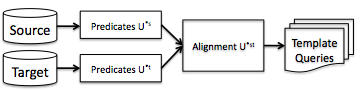
\includegraphics[scale=0.5]{p7.png}
\caption{It illustrates the overall process of generating template queries. } 
\vspace{-10pt}
\label{fig:template}
\end{figure}
 
\begin{definition} [Candidate Set]  A candidate set of an instance $s$ in $G_s$ is a instantiation of a template query with at least an attribute clause $\langle p_t,k \rangle^A$, where $k$ is in $\langle s,p_s,k \rangle \in IR(s)$
\end{definition} 

For instance, for an template query formed by the attribute clause $\langle\verb+rdf:label+,``\verb+eosinophilic+$  $\verb+pneumonia+",\sim\rangle$, where $\sim$ is one of the query types: EXACT, LIKE, AND and OR, can be expressed in SPARQL as, respectively: 

\begin{footnotesize} 
\begin{verbatim}
SELECT DISTINCT ?s  
WHERE {?s rdf:label ``eosinophilic pneumonia'' } 
 
SELECT DISTINCT ?s  WHERE {?s rdf:label ?o FILTER
regex(?0,``eosinophilic pneumonia'') } 

SELECT DISTINCT ?s  WHERE {?s rdf:label ?o FILTER 
regex(?o,``eosinophilic'')&&regex(?o,``pneumonia'')} 

SELECT DISTINCT ?s  WHERE {?s rdf:label ?o FILTER
regex(?o,``eosinophilic'')||regex(?o,``pneumonia'')} 
\end{verbatim}
\end{footnotesize}

